We propose to measure the tensor asymmetry $A_{zz}$ and tensor analyzing power $T_{20}$ from inclusive electron scattering from polarized deuterons in the quasi-elastic and elastic region of $\XMIN<x<\XMAX$, $\QMIN$~(GeV/$c)^2 < Q^2 <\QMAX$~(GeV/$c)^2$, and $\WMIN < W_{NN} < \WMAX$~GeV using the Hall C HMS and SHMS spectrometers at forward angle from a solid polarized ND$_3$ target.


\subsection{$A_{zz}$ Experimental Method} %Measurement of $A_{zz}$ }

The measured double differential cross section for electron scattering from a spin-1 target is characterized by a vector polarization $P_{z}$ and tensor polarization $P_{zz}$. With an unpolarized beam and the target field oriented along the beam, the cross section is expressed as~\cite{Leidemann:1991qs}
\begin{equation}
\frac{d^2\sigma_p}{d\Omega dE'}=\frac{d^2\sigma_u}{d\Omega dE'}\left(1+\frac{1}{2}P_{zz}A_{zz}) \right),
\label{eq:one}
\end{equation}
where $\sigma_p$ ($\sigma_u$) is the polarized (unpolarized) cross section and $A_{zz}$ is the
tensor asymmetry of the virtual-photon deuteron cross section.  This allows us to write
the polarized tensor asymmetry with positive tensor polarization using an unpolarized electron beam as
\begin{eqnarray}
\label{Azz}
A_{zz} = \frac{2}{P_{zz}}\left(\frac{\sigma_p - \sigma_u}{\sigma_u}\right).
\end{eqnarray}
The tensor polarization is given by 
\begin{equation}
P_{zz}=(p_++p_-)-2p_0,
\end{equation}
where $p_m$ represents the population in the $m_J=+1$,~$-1$,~or $0$ state.

Eq. \ref{Azz} reveals that the asymmetry $A_{zz}$ compares two different cross sections measured under different polarization conditions of the target: positively tensor polarized and unpolarized.  
To obtain the relative cross section measurement in the same configuration, the same target cup and material will be used at alternating polarization states (polarized vs. unpolarized),  and the magnetic field providing the quantization axis will be oriented along the beamline at all times.
This field will always be held at the same value, regardless of the target material polarization state. 
This process, identical to that used for the already-approved $b_1$ measurement~\cite{b1prop}, ensures that the acceptance remains consistent within the stability of the super conducting magnet.  


Since many of the factors involved in the cross sections cancel in
the ratio, Eq. \ref{Azz} can be expressed in terms 
of the charge normalized, efficiency corrected numbers of tensor polarized ($N_p$) and unpolarized ($N_u$) counts, 
\begin{eqnarray} \label{3}
A_{zz}&=&\frac{2}{fP_{zz}}\left(\frac{N_p - N_u}{N_u}\right) .
\end{eqnarray}

The dilution factor $f$ corrects for the presence of unpolarized nuclei in the target and is defined by
\begin{equation}
f=\frac{N_D\sigma_D}{N_N\sigma_N+N_D\sigma_D+\sum\limits_{A} N_A\sigma_A},
\end{equation}
where $N_D$ is the number of deuterium nuclei in the target and $\sigma_D$ is the corresponding inclusive double differential scattering cross 
section, $N_N$ is the nitrogen number of scattered nuclei with cross section $\sigma_N$, and $N_A$ is the number of other scattering nuclei of mass number $A$ with cross section $\sigma_A$. As has been noted in previous work~\cite{Frankfurt:1988nt}, the dilution factor at high $x$ drops off considerably until the SRC plateau region, as shown in Fig.~\ref{fdil}. By using a high-luminosity solid target at a small scattering angle $\theta_{e'}$, this effect will be counteracted. The dilution factor is a much smaller problem for elastic deuteron scattering at $x=2$.

\begin{figure}
\begin{center}
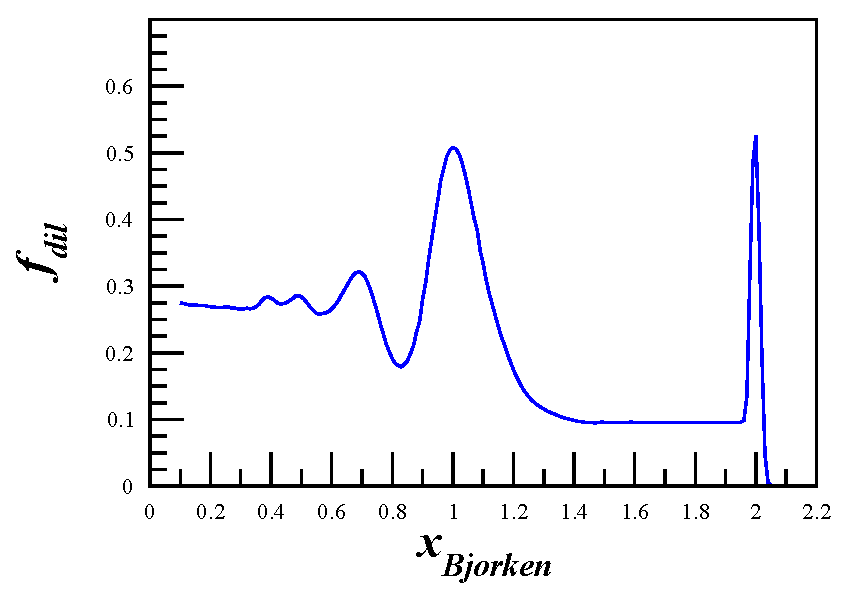
\includegraphics[width=0.45\textwidth]{figs/fdil_q2_15.eps}
\caption{\label{fdil}The estimated dilution factor, in this case at $Q^2=1.5 \mathrm{~(GeV}/c)^2$, is expected to drop off at high $x$ until it reaches the SRC plateau region and then the elastic peak at $x=2$. The low dilution factor of $1.1<x<1.95$ will be counteracted by using a high-luminosity target.}
\end{center}
\end{figure}

The dilution factor can be written in terms of the relative volume ratio of ND$_3$ to LHe in the target cell, otherwise known as the packing fraction $p_f$.  
In our case of a cylindrical target cell oriented along the magnetic field,the packing fraction is exactly equivalent to the percentage of the cell length filled with ND$_3$.  
%The dilution factor is discussed in further detail in Sec. \ref{dil}.

If the time is evenly split between scattering off of polarized and unpolarized ND$_3$, the time necessary to achieve the desired precision $\delta A$ is:
\begin{equation}
t=\frac{N_p}{R_p}+\frac{N_u}{R_u}=\frac{8}{f^2P_{zz}^2}\left(\frac{R_p(R_u+R_p)}{R_u^3}\right)\frac{1}{\delta A_{zz}^2}
\end{equation} 
where $R_{p(u)}$ is the polarized (unpolarized) rate and $N_{p(u)}$ is the total estimated 
number of polarized (unpolarized) counts to achieve the uncertainty $\delta A_{zz}$.  

%See Sec.~\ref{stat} for full details of the statistical uncertainty.
